\begin{figure}[htbp]
			\centering
			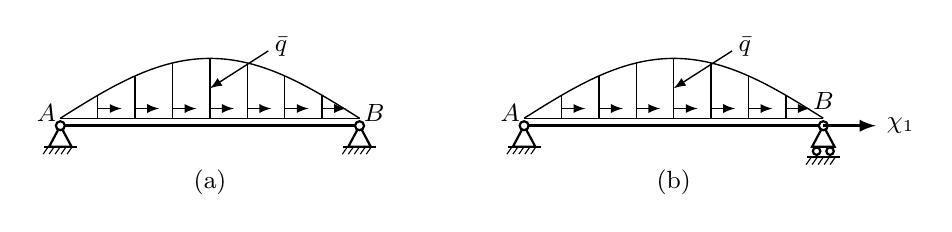
\begin{tikzpicture}[scale=0.95,>=latex,
				trave/.style={line width=1.2pt},
				carico/.style={black, line width=0.5pt},
				forza/.style={black, line width=1pt},
				]
				% ── Parametri vincoli (convenzione C06/C07) ──
				\def\tw{0.15}\def\thR{0.28}\def\rn{0.06}
				\def\rw{0.05}\def\bw{0.09}\def\gw{0.22}\def\hh{0.10}
				\def\Lb{4}        % lunghezza trave
				\def\hq{0.8}      % ordinata massima del carico (q-bar)
				\def\bb{0.10}     % quota della linea di base del carico (bordo cerniera)
				
				\def\hq{0.8}      % ordinata massima del carico (q-bar)
				\def\bb{0.10}     % quota della linea di base del carico (bordo cerniera)
				\def\fa{0.13}     % rialzo delle frecce rispetto alla linea di base
				
				% ── Cerniera in #1 ──
				\def\cerniera#1{%
					\draw[thick] (#1,0) -- (#1-\tw,-\thR) -- (#1+\tw,-\thR) -- cycle;
					\draw[thick] (#1-\gw,-\thR) -- (#1+\gw,-\thR);
					\foreach \x in {-0.16,-0.08,0,0.08,0.16}
					\draw[thin] (#1+\x,-\thR) -- ++(-0.07,-\hh);
					\draw[thick, fill=white] (#1,0) circle (\rn);}
				% ── Carrello verticale in #1 ──
				\def\carrello#1{%
					\draw[thick] (#1,0) -- (#1-\tw,-\thR) -- (#1+\tw,-\thR) -- cycle;
					\draw[thick] (#1-\bw,-\thR-\rw-0.01) circle (\rw);
					\draw[thick] (#1+\bw,-\thR-\rw-0.01) circle (\rw);
					\draw[thick] (#1-\gw,-\thR-2*\rw-0.04) -- (#1+\gw,-\thR-2*\rw-0.04);
					\foreach \x in {-0.16,-0.08,0,0.08,0.16}
					\draw[thin] (#1+\x,-\thR-2*\rw-0.04) -- ++(-0.07,-\hh);
					\draw[thick, fill=white] (#1,0) circle (\rn);}
				%			% ── Carico armonico longitudinale q(z)=qbar sin(pi z/l), verso +z ──
				\def\caricoarmonico{%
					% inviluppo (mezza sinusoide), chiuso sulla linea di base
					\draw[carico] plot[domain=0:\Lb, samples=90](\x, {\bb + \hq*sin(45*\x)});
					\draw[carico] (0,\bb) -- (\Lb,\bb);            % linea di base (chiusura)
					% ordinate (campitura): stazione centrale x=l/2 = massimo qbar
					\foreach \s in {0.5,1.0,1.5,2.0,2.5,3.0,3.5}
					\draw[carico] (\s,\bb) -- (\s, {\bb+\hq*sin(45*\s)});
					% frecce assiali, rialzate rispetto alla chiusura
					\foreach \s in {0.5,1.0,1.5,2.0,2.5,3.0,3.5}
					\draw[->, carico] (\s,{\bb+\fa}) -- (\s+0.32,{\bb+\fa});
					% q-bar (ordinata massima) con leader inclinato verso il tratto centrale
					\node[font=\small] at (2.95,{\bb+\hq+0.16}) {$\bar{q}$};
					\draw[carico, ->] (2.78,{\bb+\hq+0.10}) -- (2.0,{\bb+\hq/2});}
				
				% ===================== (a) trave incernierata =====================
				\begin{scope}[xshift=0cm]
					\draw[trave] (0,0) -- (\Lb,0);
					\cerniera{0}\cerniera{\Lb}
					\node[above left=-2pt, font=\small]  at (0,0)    {$A$};
					\node[above right=-2pt, font=\small] at (\Lb,0)  {$B$};
					\caricoarmonico
					\node[font=\small] at (\Lb/2,-0.75) {(a)};
				\end{scope}
				
				% ===================== (b) sistema principale =====================
				\begin{scope}[xshift=6.2cm]
					\draw[trave] (0,0) -- (\Lb,0);
					\cerniera{0}\carrello{\Lb}
					\node[above left=-2pt, font=\small] at (0,0) {$A$};
					\node[above=1pt, font=\small] at (\Lb,0.05) {$B$};
					\caricoarmonico
					\draw[->, forza] (\Lb,0) -- (\Lb+0.7,0);    % forza iperstatica
					\node[right, font=\small] at (\Lb+0.72,0) {$\chi_1$};
					\node[font=\small] at (\Lb/2,-0.75) {(b)};
				\end{scope}
				
			\end{tikzpicture}
			\caption{a)~trave incernierata con carico armonico longitudinale;
				b)~sistema principale scelto, con la cerniera in $B$ sostituita
				da un carrello verticale e dalla forza iperstatica $\chi_1 = H_B$.}
			\label{fig:stat_iper_long_01}
		\end{figure}
